\section{An overview on the search and the best-fit template }
Generally, a GW signal from a CBC event is expected to be buried in the detector noise and a careful data analysis needs to be performed to extract the information of the signal from the detector data. Multiple GW search pipelines are developed equipped with various algorithms and techniques to detect the GW signal from the detector noise \cite{GSTLAL1,GSTLAL2,Canton:2014ena,Usman:2015kfa,Nitz:2017svb}.  

In this chapter, the specific GW search pipeline we refer to is called \textbf{PyCBC}, which is an open source software package that has inbuilt algorithms to detect and analysis CBC events from the calibrated detector data [For the details of PyCBC search pipeline refer to \cite{Usman:2015kfa}]. The search relies on a  technique known as \textit{matched filtering} \cite{SchutzBF, JCreightonBook}. The basic idea in match filtering is to 'match' (or compare) the data from the detector to the expected GW waveform, often times referred to as templates. Waveforms are obtained by solving the Einsteins equation either using a variety of analytical approximations or numerically or with a combination of both analytical and numerical techniques.  Each variant of obtaining the templates corresponds to a \textit{waveform family} or an \textit{approximant}.

Mathematically, the operation of match filtering can be written down as a weighted inner product in the frequency domain,
\begin{align}
\mathcal{M}(t) = \left\langle s(f)| h(f) \right\rangle = 4 \mathrm{Re} \int^{f_{high}}_{f_{low}} \frac{s(f) h^{*}(f) e^{2 \pi \iota f t}}{S_{n}(f)} df
\end{align}
Here, $s(f)$ is the signal contained in the data, h(f) is the template and $S_{n}(f)$ is the one-sided PSD and is defined by averaging over the noise realization and is given as,

\begin{align}
\left\langle s(f)s(f') \right\rangle = \frac{1}{2} S_{n}(f) \delta(f-f') 
\end{align}
Then detection statistic called \textit{new-SNR} is then constructed by re-weighting the match filter value and combining the values obtained from each of the detector data [for details of the detection statistic used in LIGO search refer to \cite{newSNR1,newSNR2,FindChirp,Usman:2015kfa}].  

Furthermore, when a GW signal from a CBC event is present in the data, one does not a priori know the parameters of the compact binary system. Therefore, a bank of templates (technically called \textit{template-bank}) is created and the data is matched against each template in this bank \cite{FindChirp}. In the search pipeline, PyCBC, the template bank corresponds to waveform emitted by CBC whose component spins are aligned/anti-aligned to the orbital angular momentum of the system (the bank is called an aligned spin bank). Further, the binaries are assumed to have negligible eccentricity. When constructing the template bank, one needs to sample the astrophysical parameter space sufficiently densely to be able to capture the GW signal with sufficient SNR but also keep the bank sparse enough that it is computationally efficient. In PyCBC the template bank is generated such that no more than 3\% SNR is lost due to the discreteness of the template bank. When a match-filter operation is performed throughout this bank, the search pipeline reports the parameters of the template that produced the maximum match as the \textit{best-fit-template}. This parameter gives an approximate estimate of the astrophysical parameter and a further careful parameter estimation study is followed to infer the true parameters of the system. Note that the best-fit template parameter will depend on the state of the detector at the time of the event, on the family of templates being used and the discreteness of the bank chosen. 

\section{On the detection of GW150914}

On 14th September 2015, both the LIGO detectors recorded a GW signal consistent with what GR would predict when two BHs with masses $\sim 36\Msun$ and $29\Msun$ inspiraled and merged \cite{gw150914detection,gw150914search}. The PyCBC was one of the search pipelines employed by the LIGO collaboration to detect the signal. For reporting the statistical confidence of this detection, the data from a total coincident observation time of $16$ days \footnote{after applying the data quality vetoes details of which can be found in \cite{gw150914vetos}}  was used for the analysis. From this data, a noise background equivalent to 608000 years was produced by performing unphysical time delay; time shifts greater than 10 milliseconds (greater light travel time between the dectector) ensure that the simulate data stream has no real astrophyical signal in it and contains only detector noise realization. The statistic used by the LIGO collaboration for detection is an empirically re-weighted combined SNR detail of which can be found in \cite{detectionStat1}. On analysing the data containing GW150914 event, it was found that this event has a combined SNR of 23.6. The false alarm probability was calculated to be $\sim 2 \times 10^{ -7}$, which affirms that the signal corresponded to an astrophycial source and not a noise mimiker.The statistical significance of this event was reported to be 5.1 $\sigma$. It should be emphasised that this event was exceptionally loud. 

Further, in Table \ref{tab:best-fitGW150914}, we list the best-fit parameters reported by the PyCBC search. It should be reiterated that these parameters are approximate parameters but it is obtained in low latency. The values of best-fit-template parameter reported by the search differ from the parameters inferred on performing a careful Bayesian parameter estimation (compare Table \ref{tab:best-fitGW150914} with results presented in papers \cite{gw150914PE}). The study presented in section \ref{sec:dirrect-comparision} was performed very shortly after the GW150914 trigger was recorded. At that time, the parameter estimation studies were still being performed and the PE inferred values were not available. Therefore in the study presented in section \ref{sec:dirrect-comparision}, we use the best-fit-template parameters presented in table \ref{tab:best-fitGW150914}.


\begin{table}[h!]
\centering
\begin{tabular}{@{}|c|c|@{}}
\toprule
mass 1                   & 49.9          \\ \midrule
mass 2                   & 36.6          \\ \midrule
spin 1z                  & 0.96          \\ \midrule
spin 2z                  & -0.89         \\ \midrule
Effective Distance in L1 & 1194.9118 Mpc \\ \midrule
Effective Distance in H1 & 970.70534 Mpc \\ \midrule
Arrival Phase in L1      & 0.58 rad      \\ \midrule
Arrival Phase in H1      & -2.77 rad     \\ \bottomrule
\end{tabular}
\caption{In this table we summarize the parameters of the best-fit-template reported by the search pipeline PyCBC on analyzing the data containing the vent GW150914. These values are used in the study presented in section \ref{sec:dirrect-comparision}}.
\label{tab:best-fitGW150914}
\end{table}

\section{Direct comparison of the data and best fit template}
\label{sec:dirrect-comparision}`
The exceptionally loud nature of GW150914 trigger prompted us to look at the raw data from the detectors directly, unlike in the case of search pipelines where one is more concerned about the SNR timeseries for the events.  In this section, we describe our preliminary analysis on the raw data containing the GW150914 trigger.  The basic premise of this work was to check for visual consistency between the observed signal and the best-fit template reported by the search pipeline.

The raw GW strain seen by the LIGO detectors are recorded in a channel called the GDS-CALIB-STRAIN. The data in this channel is calibrated but no other data quality vetoes are applied. We use the timeseries recorded in this channel and perform a minimal set of filtering needed to visually see the GW event. Firstly, the sensitivity of the detectors are not uniform across all frequencies in its band and the sensitivity to frequencies is encoded in the PSD.  Therefore, to remove this feature, we 'whiten' the data by applying an inverse noise amplitude spectrum to the data in the fourier domain.  Moreover, the data needs to be band passed to remove contaminants in frequencies that the detector is not sensitive to. Furthermore, the detector data contains known noise contaminations that are localized in frequency. One such noise contamination comes due to the electric power line and is localized at frequencies that are harmonics of 60 Hz. In order to see the signal, we have to notch out these power-line frequencies from the data. We do this using an analytical filter constructed using a zero-pole-gain (zpk-filter) model that notches out the power-line frequencies. The filter is depicted in the bottom right inlay panel of figure \ref{fig:overlayGW150914}. The filter is designed such that the amplitude is set to 1 at 100 Hz. Next, the data is filtered both forward and then backwards to ensure that filtering does not introduce a phase error (zero-phase filtering).  Note that the filter is acausal (specifically, symmetric in time) and is designed to introduce a zero-phase offset. The impulse response of the filter can be seen in the top right inlay panel of figure \ref{fig:overlayGW150914}. At this point, it must be emphasised that these set of filtering are very non-aggressive and minimal data conditioning that we perform in order to visually examine the data. 

Next, we describe the process we use to align the data from the two detectors with each other and to the best fit template. From the search pipeline, one can find the time at which the SNR peaks in each of the detector data. This corresponds to the time when the template aligns best with the data. However, note that the  value of this timestamp may vary slightly when the search is performed using the different template families (also known as waveform approximants) ;they depend on the convention of defining the $t_{merger}$ within the waveform family. In our study, we find that this difference in the timestamps reported when a search is performed with different waveform family can affect the alignment of the template with the data. 

In order to overlay the best-fit template on to the detector data timeseries, one would need a time-domain template with the best-fit-templateparameters. However, typically the search uses a frequency domain template in order to increase computational efficiency. For this study, we construct a template bank consisting of a single time-domain template corresponding to the parameter described in Table \ref{tab:best-fitGW150914}. The template family used in our study corresponds to a spinning effective one body waveform (called the SEOBNRv2 approximant in the LAL code library)  \cite{SEOBNRv2}. We then perform a search on the data containing the event using this single-template template bank and record the reported time of the merger. This reported time of merger is used to align the raw data from the two detectors. Furthermore, it is also used to align the best-fit template to the data to produce the overlay plot presented in Figure \ref{fig:overlayGW150914}. The merger times we obtain in our study are listed below in Table \ref{tab:arrival-time}.


\begin{table}[]
\centering
\begin{tabular}{|c|c|}
\hline
Detector & Time (in sec)        \\ \hline
L1       & 1126259462.415039062 \\
H1       & 1126259462.422363281 \\ \hline
\end{tabular}
\caption{This table presents the time at which SNR timeseries peaks in each of the detector. The detector data is matched to a timedomain template (SEOBNRv2) corresponding to the best-fit-template parameters reported by the PyCBC search.}
\label{tab:arrival-time}
\end{table}

This corresponds to a time delay of 7.32 ms between the Livingston (L1) and Hanford (H1) detectors. Our analysis uses a sampling rate of 16384Hz and therefore, to align the data from the two detectors, we shift the raw data of H1 by 120 sample points. Also note that, the data is also appropriately phase shifted to obtian alignment presented in Figure \ref{fig:overlayGW150914}.

\begin{figure*}
\subfloat{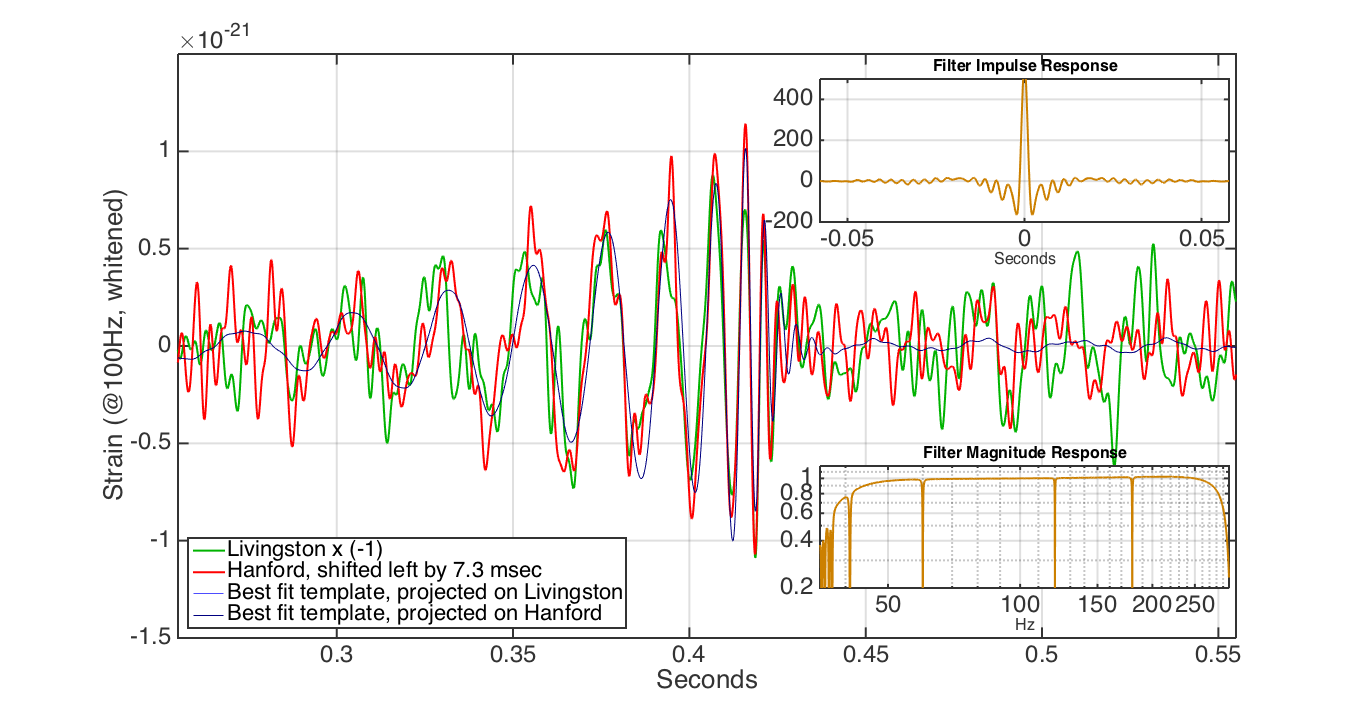
\includegraphics[width=\textwidth]{figures/overlayGW150914.png} }
\caption{Direct comparison of the detector data with the best fit template. The data from the H1 and L1 have been minimally filtered and  appropriately shifted to align with each other. The best fit template corresponding to each of the detector timeseries is overlayed on the data. The inlay panel display the details of the filters used to condition the data}
\label{fig:overlayGW150914}
\end{figure*}

The result of this study is presented in Figure \ref{fig:overlayGW150914}. We see an excellent agreement between the raw data from the two detectors (see the coherence in the green and the red curve in the main panel). Furthermore, note that the best-fit-template (the thin blue and black lines) match very well with the two detector data (and with each other). In this plot we see that a minimal set of non-agressive filtering allows us to clearly see the inspiral and merger phase of the GW signal buried in the detector noise. However, the ringdown portion of the waveform is buried under the noise floor. 

A refined version of Figure \ref{fig:overlayGW150914} was prepared by the LIGO collaboration and is presented in the top two panels of Figure 1 in the GW150914 detection paper \cite{gw150914detection}. For the easy of comparision, we present this plot in Figure \ref{fig:Fig1GW150914detection}. Figure \ref{fig:Fig1GW150914detection} differs from Figure \ref{fig:overlayGW150914} in the following ways. \textbf{Ask Duncan for details of producing the Figure 1 of the GW150914 detection paper, especially the filtering done.}




\begin{figure*}
\subfloat{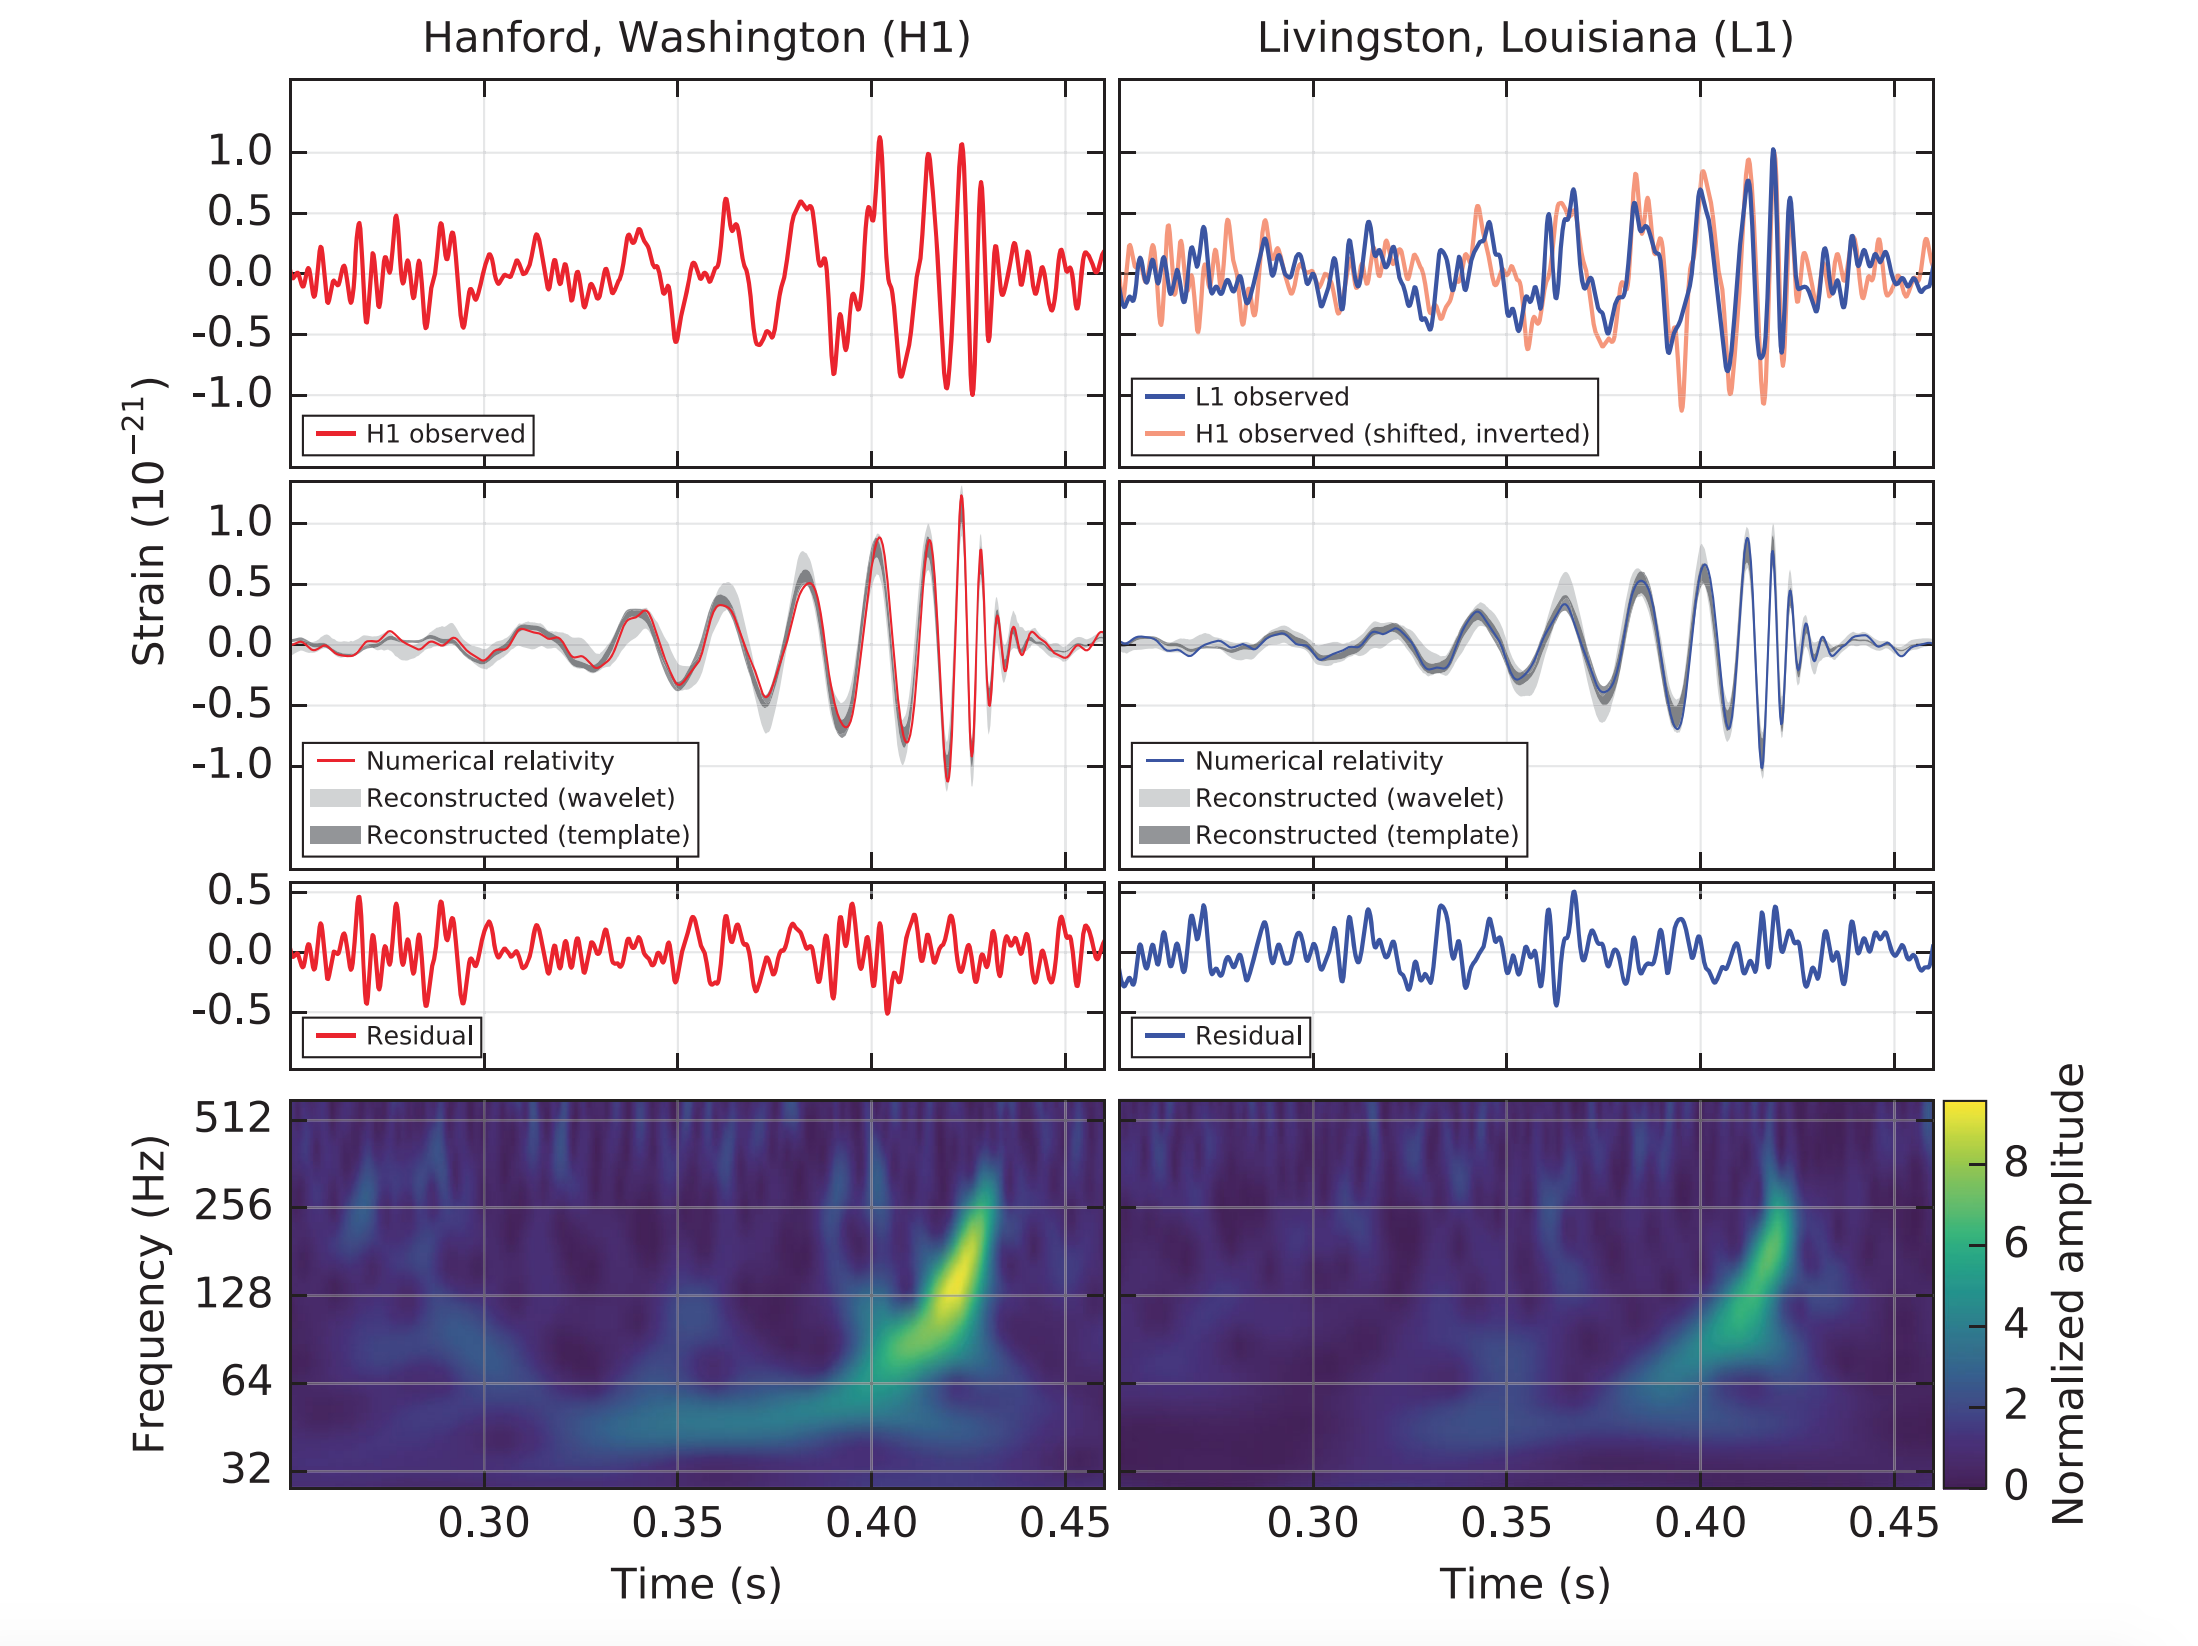
\includegraphics[width=\textwidth]{figures/dectionPaperFig1.png} }
\caption{Figure 1 from GW150914 detection paper. This figure is taken from the GW150915 detection paper \cite{gw150914detection} by the LIGO collaboration. The top two panels of this figure shows a more refined versino of the plot we produce in our preliminary study presented in Figure \ref{fig:overlayGW150914}.}
\label{fig:Fig1GW150914detection}
\end{figure*}

\section{Parameters of GW150914 inferred using SEOBNRv3 waveform family}

Having emphasised that the parameters reported by the search are approximate and a careful PE needed to be followed in order to estimate the astrophysical parameters, in this section we briefy summarize the parameters estimate for GW150915 using a template family that models spinning and precessing BBH waveforms in an effective one body formulation. This section contains results of the PE studies perfromed by the LIGO collaboration that are presented in papers \cite{gw150914PE} and \cite{gw150914PEseobnrv3}.  

PE of GW150914 was initially performed using two template families that had independent ways of computing the waveforms \cite{gw150914PE}. The two template families were a) One of the template families used was based on an effective one body (EOB) formulation and is calibrated to a set of numerical relativity simulation. This model did not allow for a non-aligned spin, thereby did not contain precession physics in the waveform modelling. In the LAL code library, the implementation of this template family is called SEOBNRv2  \cite{SEOBNRv2}.  Further,  to perform the PE study present in \cite{}, an implementation of the reduced ordered model of this waveform in the frequency domain, called the SEOBNRv2-ROM-DoubleSpin,  was used in view of computational efficiency.  b) The second waveform family used in the PE study presented in \cite{gw150914PE}, models the waveform by phenomenologically predicting the amplitude and phase evolution.  This waveform family is also calibrated to a set of numerical relativity simulations. Furthermore, in this waveform family, the precession physics of the binary system is incorporated (i.e) it can generate waveform corresponding to non-aligned binary black hole systems.  In the LAL code library,  the implementation of this waveform family is called as IMRPhenomPv2  \cite{IMRPhenomPv2}. 

The primary reason that the LIGO collaboration performed the PE studies of the GW150914 event using two independent template families was to understand the effect of waveform systematics in the inferred astrophysical parameters of the system \cite{gw150914PE}. It was then anticipated that the difference in the inferred parameters arising due to the difference in the waveform family will be on the pessimistic end, as we apriori know that SEOBNRv2 lacks the precision physics in it. Therefore, an implementation of effective one body template family that incorporated the precession physics was developed shortly after the initial parameter estimation analysis presented in \cite{gw150914PEseobnrv3}. The new implementation of precessing EOB waveform family was called SEOBNRv3  and the details of the physics in modelling this waveform can be found in \cite{SEOBNRv3}. I was involved in the review process of the implementation of this waveform family in the LAL code library.  Table \ref{tab:PEwithSEOBNRV3} presents the parameter estimation results obtained by the LIGO collaboration using the SEOBNRv3 template family. It was found that the inferred parameters of GW150914 using the two precision models were indeed very close, affirming that inferred astrophysical parameters of the system are not affected significantly by the difference in the waveform models. Further, the difference in inferred astrophysical parameters due the difference in waveform family used for performing the PE study is beautifully visualized in Figure 1 of \cite{gw150914PEseobnrv3}. 

\begin{table}[]
\centering
\begin{tabular}{ll}
1 & 1 \\
0 & 0
\end{tabular}
\caption{Place holder table: this will contain colomn 1 and 2 od table in 1 in \cite{gw150914PEseobnrv3} exactly.}
\label{my-label}
\end{table}




%%%%%%%%%%%%%
% On 14th September 2015, both the LIGO detectors recorded a GW signal consistent with what GR would predict when two BHs with masses $\sim 36 \Msun$ and $29 \Msun$ inspiraled and merged \cite{gw150914detection}. For reporting the statistical confidence of this detection, the data from a total coincident observation time of $16$ days \footnote{after applying the data quality vetoes}  was used for the analysis. From this data, a noise background equivalent to 608000 years was produced by performing unphysical time delays. The statistic used by the LIGO collaboration for detection is an empirically re-weighted combined SNR details of which can be found in \cite{detectionStat1}. On analysing the data containing GW150914 event, it was found that this event has a combined SNR of 23.6 and a false alarm probability of $\sim 2 \times 10^{-7}$. The statistical significance of this event was reported to be 5.1 $\sigma$.

% GW150914 was an extraordinarily loud event. It could be visually seen after performing just some basic filtering on the raw detector data. In section \ref{sec:dirrect-comparision}, we present a direct comparison of the raw data from the detectors (with minimal non-aggressive filtering) overlayed with a GR predicted BBH template \footnote{The models of GWs that are used in matched filtered searches are calleed as templates.}. The template corresponds to a BBH system with parameters reported by the search pipeline. In this study we see that there is a visual consistency between the observed data and the best-fit template reported by the seach pipeline.

% Although the search pipeline reports a rough estimate of the BBH parameters, a careful Bayesian parameter estimation needs to be carried to extract the astrophysical parameters of the system. In section \ref{sec:prop-GW150914}, we summarize the astrophysical parameters of GW150914 inferred by the LIGO collaboration. This section attempts to highlight a few points from \cite{gw150914PE} and \cite{gw150914PEseobnrv3}.

% \section{Direct comparison of the data and best fit template}
% \label{sec:dirrect-comparision}
% In this section, we describe a priliminary analysis done soon after the detection of GW150914. The basic premise of this work was to check for visual consistency between the observed signal and the best-fit template reported by the search pipeline. A more refined version of this study was performed by the LIGO collaboration and is presented as Figure 1 of \cite{gw150914detection}.

% \subsection{Filtering the data}
% The raw GW strain seen by the LIGO detectors are recorded in a channel called GDS-CALIB-STRAIN. The data in this channel is calibrated but no other data quality vetoes are applied. We use the timeseries recorded in this channel and perform a minimal set of filtering needed to visually see the GW event. We first whiten the data (i.e) apply inverse detector power spectral density (PSD) curve. Then, the data is band passed and the harmonics of power-line frequencies are notched out using an analytical zero-pole-gain(zpk) filter. The filter is depicted in the bottom right inlay panel of figure \ref{fig:overlayGW150914}. The filter amplitude is set to 1 at 100 Hz. The data is filtered forward and backward to ensure that filtering does not introduce a phase error. Further, the filter is acausal (specifically, symmetric in time) and is designed to introduce zero-phase offset. This can be seen in the top right inlay panel of figure \ref{fig:overlayGW150914}.

% \subsection{Best-fit template parameters}
% The search pipeline used to detect CBC signals is based on matched filtering the detector data against the expected GW templates. A template bank is created and for each template in this bank, a match filtered operation is carried out. The parameters of the tempate that maximizes match is reported by the pipeline as the best fit parameter.

% Below, we enlist the parameters of the best-fit template reported by the search pipeline PyCBC obtained by analyzing the streach of 
% data containing GW150914. We use these parameters both for  generating andthe for  aligning the best-fit template on the raw data from the detector to produce figure \ref{fig:overlayGW150914}.


% \begin{itemize}
% \item m1=47.9 $\Msun$
% \item m2=36.6 $\Msun$
% \item s1=0.96
% \item  s2=-0.89
% \item Effective distance
%     \begin{itemize}
%     \item L1: 1194.9118 Mpc
%     \item H1: 970.70534 Mpc
%     \end{itemize}

% \item Template phase
%     \begin{itemize}
%     \item L1: 0.58 radians
%     \item H1: -2.77 radians
%     \end{itemize}
% \item Ringdown parameters
%     \begin{itemize}
%     \item f=228Hz
%     \item Q=3.651
%     \end{itemize}

% \end{itemize}

% \subsection{Aligning the data and the template}

% The search pipeline reports the peak of the SNR time series as the merger time. Note that this time may vary slightly when the search is performed using the different template families (also known as waveform approximants) and depends on the convention of defining the $t_{merger}$ in the waveform family. In order to overlay the best-fit template on to the detector data time series, one would need a time-domain template with appropriate parameters. However, typically the search uses a frequency domain template in order to increase computational efficiency. For this study, we construct a template bank consisting of a single time-domain template corresponding to the parameter described above (i.e) the best-fit parameter reported by the search. We then perform a search on the data containing the event using this single-template template bank and record the reported time of the merger. This reported time of merger is used to align the raw data from the two detectors. Furthermore, it is also used to align the best-fit template to the data to produce the overlay plot presented in figure \ref{fig:overlayGW150914}. The merger times we obtain in our study are listed below.

% \begin{itemize}
% \item L1: 1126259462.415039062 sec
% \item H1: 1126259462.422363281 sec.
% \end{itemize}

% This corresponds to a time delay of 7.32 ms between the Livingston (L1) and Hanford (H1) detector. Our analysis uses a sampling of 16384Hz and therefore, to align the data from the two detectors, we shift the raw data of H1 by 120 sample points. The data is also appropriately phase shifted to obtian alignment presented in Figure \ref{fig:overlayGW150914}.

% From Figure \ref{fig:overlayGW150914} we find a visual agreement between the raw detector data and the best-fit template reported by the search pipeline. We can see that the data from the two detectors can be coherently aligned in phase with each other and also with the best-fit template.

% \begin{figure*}
% \subfloat{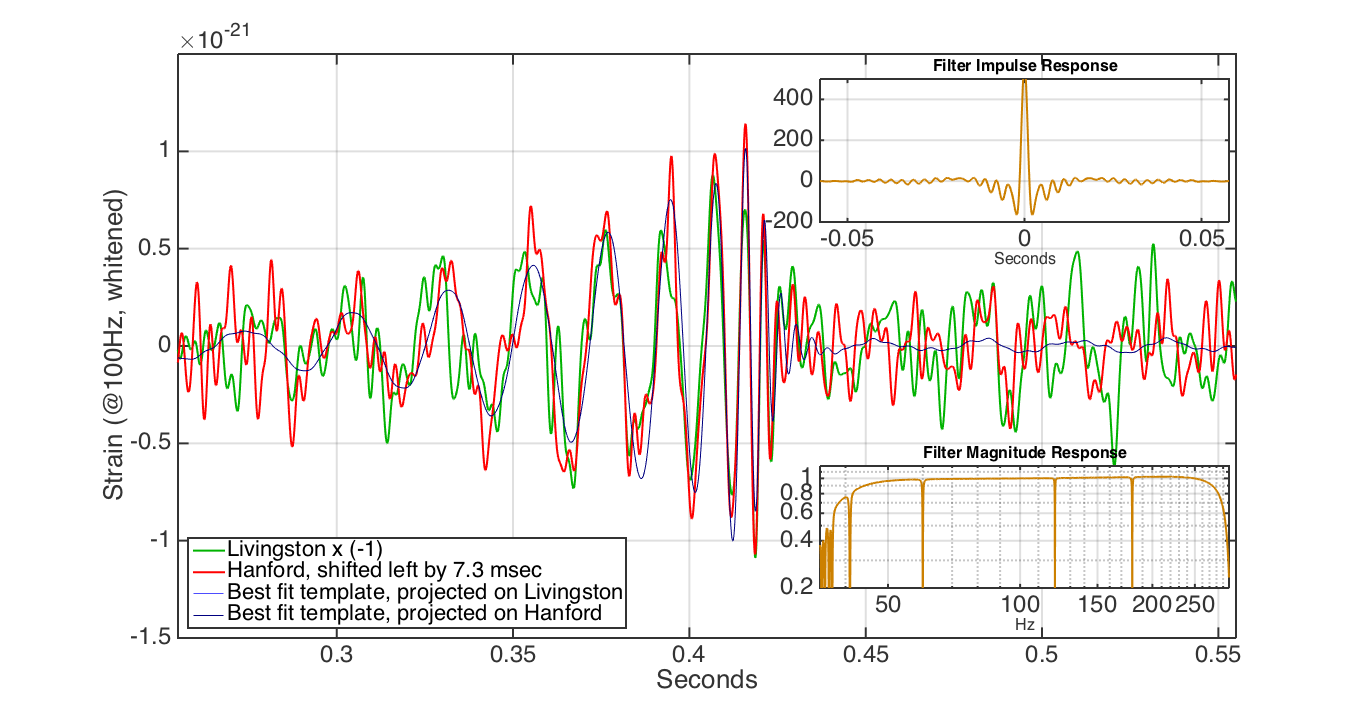
\includegraphics[width=\textwidth]{figures/overlayGW150914.png} }
% \caption{Direct comparison of the detector data with the best fit template. The data from the H1 and L1 have been minimally filtered and  appropriately shifted to align with each other. The best fit template corresponding to each of the detector timeseries is overlayed on the data. The inlay panel display the details of the filters used to condition the data}
% \label{fig:overlayGW150914}
% \end{figure*}






